%preamble
\documentclass{article}
\usepackage[paperheight=8cm,paperwidth=20cm,margin=5mm]{geometry}
\usepackage{graphicx}
\usepackage{tikz}
\usepackage{calc}
\usepackage[justification=centering]{caption}
\pagestyle{empty}
\input ean13

\setlength{\parindent}{0pt}
\setlength{\parskip}{0pt}
\setlength{\tabcolsep}{2pt}
\renewcommand{\arraystretch}{0.95}

\newcommand{\panelsep}{\vspace{4mm}}

\begin{document}
\noindent
\begin{minipage}[t][6cm][s]{0.32\textwidth}\vspace{0pt}
\sffamily\small
\textbf{Ingredients:} nan

\vfill
\begin{flushleft}
\begin{tikzpicture}[baseline]
\node[anchor=south west] at (0,0){{\EANnan}\relax};
\end{tikzpicture}
\vspace{-4mm}
\large\bfseries nannan 
\large\bfseries nan
\end{flushleft}
\end{minipage}\hfill%
\begin{minipage}[t][6cm][c]{0.32\textwidth}\vspace{0pt}
\centering

\includegraphics[width=4cm]{brand-logo.png}

\vspace{1.5mm}
{\sffamily\bfseries\fontsize{16}{18}\selectfont nan\par}
\end{minipage}\hfill%
\begin{minipage}[t][6cm][s]{0.32\textwidth}\vspace{0pt}
\raggedright\small
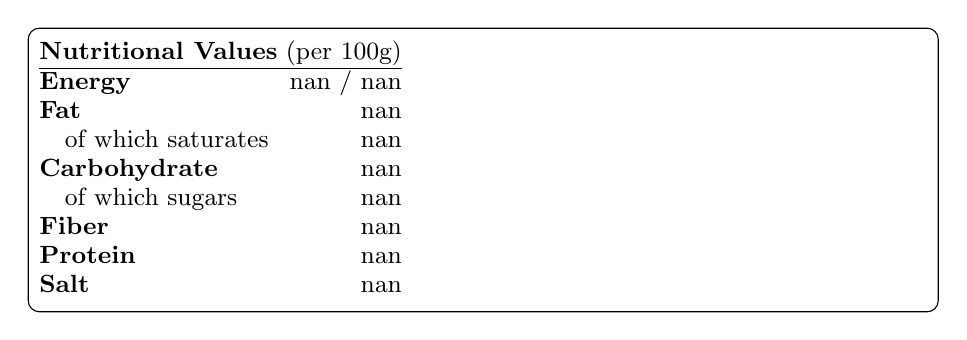
\begin{tikzpicture}
\node[draw,rounded corners=4pt,line width=0.4pt,inner sep=4pt,outer sep=0pt,anchor=north west] (box) at (0,0) {%
\begin{minipage}{0.93\linewidth}
\small
\begin{tabular}{@{}l r@{}}
\multicolumn{2}{@{}l@{}}{\textbf{Nutritional Values} \hfill (per 100g)} \\ \hline
\textbf{Energy} & nan / nan \\
\textbf{Fat} & nan \\
\quad of which saturates & nan \\
\textbf{Carbohydrate} & nan \\
\quad of which sugars & nan \\
\textbf{Fiber} & nan \\
\textbf{Protein} & nan \\
\textbf{Salt} & nan \\
\end{tabular}
\end{minipage}};
\end{tikzpicture}

\vspace{1cm}
\sffamily\footnotesize
nan

\vspace{3mm}
Best Before nan
\end{minipage}
\end{document}